\documentclass{report}

% Language setting
% Replace `english' with e.g. `spanish' to change the document language
\usepackage[english]{babel}

% Set page size and margins
% Replace `letterpaper' with `a4paper' for UK/EU standard size
\usepackage[letterpaper,top=2cm,bottom=2cm,left=3cm,right=3cm,marginparwidth=1.75cm]{geometry}

% Useful packages
\usepackage{amsmath}
\usepackage{graphicx}
\usepackage[colorlinks=true, allcolors=blue]{hyperref}

\title{High Performance Computing Project - A.A. 2022/2023}
\author{Andres Bermeo Marinelli}

\begin{document}
\maketitle
\tableofcontents
\chapter{Benchmarking MKL, OpenBLAS, and BLIS}
\section{Introduction}
In this exercise we compare the performance of three High Performance Libraries
(HPC): MKL, OpenBLAS, and BLIS. In particular, we focus on the level 3 BLAS 
function called \texttt{gemm}, which multiples an $m \times k$ matrix $A$ times 
a $k \times n$ matrix $B$ and stores the result in an $m \times n$ matrix $C$. 

This function comes in two types, one for single 
precision (float) and the other for double precision (double). Furthermore, it 
is capable of exploiting paralellism using OpenMP (OMP) to speed up the 
calculations, provided that we have the required computational resources.

Using squared matrices only, we perform a scalability study in two scenarios. 
In the first scenario, we fix the number of cores, and increase the size of the
matrices from $2000$ to $20000$. In the second scenario, we fix the matrix size 
to $10000$ and increase the number of cores that \texttt{gemm} can use by 
modifying the \texttt{OMP\_NUM\_THREADS} environment variable.

In both scenarios, we repeat the measurements for both single and double
precision, for both THIN and EPYC nodes, using the maximum number of cores.

Furthermore, for the second scenario, we also modify the thread affinity policy 
of OMP in order to observe any differences.

\section{Methodology}
\subsection{Compiling BLIS and obtaining binaries}

We begin by downloading the BLIS library by using the following commands:
\begin{verbatim}
    $git clone https://github.com/flame/blis.git
    $cd blis
    $srun -p {NODE} -n1 ./configure --enable-cblas --enable-threading=openmp --prefix=/path/to/myblis/lib auto
    $srun -p {NODE} -n 1 --cpus-per-task={P} make -j {P}
    $make install
\end{verbatim}
Where \texttt{NODE} can be specified as either \texttt{THIN} or \texttt{EPYC} and 
\texttt{P} are the available cores for each node, $24$ and $128$ respectively.

With these commands, we have compiled the BLIS library for the desired 
architecture.

Next, we specify the flag in the Makefile to compile for float or double using 
\texttt{\-DUSE\_FLOAT} or \texttt{\-DUSE\_DOUBLE}. Then, we run:
\begin{verbatim}
    $salloc -n {P} -N1 -p {NODE} --time=1:0:0
    $module load mkl/latest
    $module load openBLAS/0.3.23-omp
    $export LD_LIBRARY_PATH=/path/to/myblis/lib:$LD_LIBRARY_PATH
    $srun -n1 make cpu
\end{verbatim}
Which will generate the binaries for the desired architecture, with floar or 
double precision, depending on the flag we used.

To run, we use: 
\begin{verbatim}
    $srun -n1 --cpus-per-task=128  ./gemm_mkl.x {size_M} {size_K} {size_N}
    $srun -n1 --cpus-per-task=128  ./gemm_oblas.x {size_M} {size_K} {size_N}
    $srun -n1 --cpus-per-task=128  ./gemm_blis.x {size_M} {size_K} {size_N}
\end{verbatim}

At the end of this procedure, we should have the appropriate binaries for each 
architecture, and for each type of precision, double or float.

We now detail the steps to obtain the measurements for both scenarios.

\subsection{Using a fixed number of cores}

For this section, we use all the cores available in a THIN or an EPYC node: 24 
and 128, respectively. 

Since we only use squared matrices, we can describe the dimensions of the matrices 
with a single number, which we call "size". 

For both architectures, we start with a size of $2000$ and end with a size of 
$20000$, with jumps of $2000$ for a total of $10$ sizes. For each size, 
we repeat the measurement $10$ times and report the average and standard 
deviation.

Finally, we repeat the measurements for both floating point precision and double 
point precision.

The scripts that were used can be found in the folder \texttt{exercise2/scripts}, 
under the name \texttt{es2\_1\_thin.sh} and \texttt{es2\_1\_epyc.sh}.

It is important to observe that in this section, since we are using the entire 
node, there is little possibility to play with combinations of thread affinity.

This will be done for the next section.

Furthermore, contrary to the guidelines for the exercise, we decided to use the 
entire node to benchmark its full capacity, and also to avoid wasting 
resources. 

In fact, to obtain an accurate benchmark, we need to reserve the whole node, 
regardless of the number of cores we decide to use. This is because if other 
people began to use the other half of the node, this could introduce additional 
workloads which interfere with the benchmark. 

\subsection{Using a fixed matrix size}

For this section, we fix the size of the matrices to $10000$. Then, we slowly 
increase the number of cores to be used, until we reach the maximum. 

To set the number of cores, we change the environment variable 
\texttt{OMP\_NUM\_THREADS} to the desired value.

For THIN nodes, which have $24$ cores, we start using $1$ core, then $2$ and 
then we increase by steps of $2$, for a total of 13 points.

For EPYC nodes, which have $128$ cores, we start from $1$, then $10$ and then 
we increase by steps of $10$ until $120$. We also use $128$ cores, to see what 
happens at full capacity. We obtain a total of $14$ points.

We repeat all measurements $10$ times and report the average and standard 
deviation.

As usual, we repeat this process for both floating and double point precision.

In this section, we have the liberty to explore different thread allocation 
policies since we are not always using the whole node. 

We decided to use following combinations:
\begin{enumerate}
    \item \texttt{OMP\_PLACES=cores} and \texttt{OMP\_PROC\_BIND=close} 
    \item \texttt{OMP\_PLACES=cores} and \texttt{OMP\_PROC\_BIND=spread} 
\end{enumerate}

The scripts that were used can be found in the folder \texttt{exercise2/scripts}, 
under the names \texttt{es2\_2\_close\_thin.sh}, \texttt{es2\_2\_close\_epyc.sh}, 
\texttt{es2\_2\_spread\_thin.sh}, and \texttt{es2\_2\_spread\_epyc.sh}.


\section{Results and Discussion}
\section{Conclusion}
\chapter{Conway's Game of Life}


\section{Introduction}

Your introduction goes here! Simply start writing your document and use the Recompile button to view the updated PDF preview. Examples of commonly used commands and features are listed below, to help you get started.

Once you're familiar with the editor, you can find various project settings in the Overleaf menu, accessed via the button in the very top left of the editor. To view tutorials, user guides, and further documentation, please visit our \href{https://www.overleaf.com/learn}{help library}, or head to our plans page to \href{https://www.overleaf.com/user/subscription/plans}{choose your plan}.

\section{Some examples to get started}

\subsection{How to create Sections and Subsections}

Simply use the section and subsection commands, as in this example document! With Overleaf, all the formatting and numbering is handled automatically according to the template you've chosen. If you're using the Visual Editor, you can also create new section and subsections via the buttons in the editor toolbar.

\subsection{How to include Figures}

First you have to upload the image file from your computer using the upload link in the file-tree menu. Then use the includegraphics command to include it in your document. Use the figure environment and the caption command to add a number and a caption to your figure. See the code for Figure \ref{fig:frog} in this section for an example.

Note that your figure will automatically be placed in the most appropriate place for it, given the surrounding text and taking into account other figures or tables that may be close by. You can find out more about adding images to your documents in this help article on \href{https://www.overleaf.com/learn/how-to/Including_images_on_Overleaf}{including images on Overleaf}.

\begin{figure}
\centering
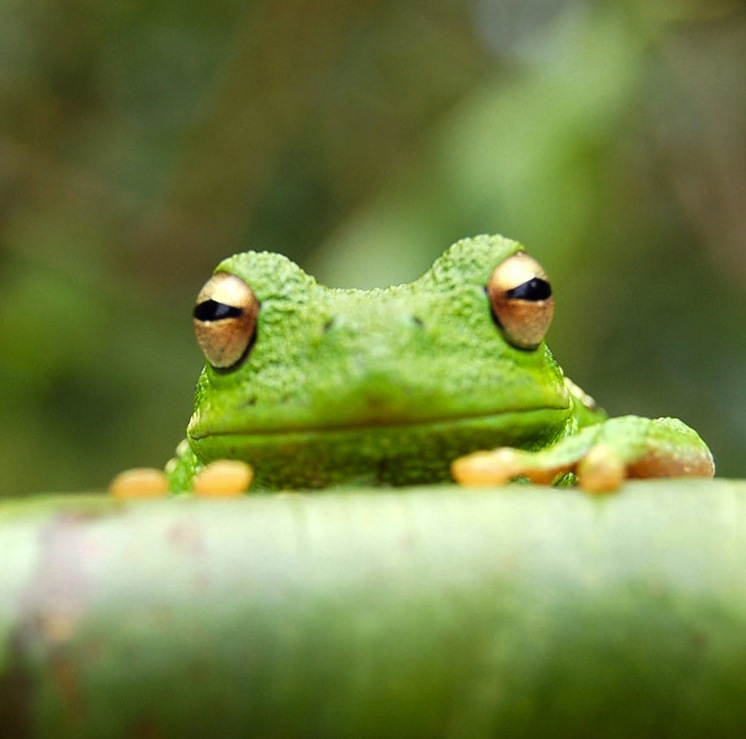
\includegraphics[width=0.25\linewidth]{frog.jpg}
\caption{\label{fig:frog}This frog was uploaded via the file-tree menu.}
\end{figure}

\subsection{How to add Tables}

Use the table and tabular environments for basic tables --- see Table~\ref{tab:widgets}, for example. For more information, please see this help article on \href{https://www.overleaf.com/learn/latex/tables}{tables}. 

\begin{table}
\centering
\begin{tabular}{l|r}
Item & Quantity \\\hline
Widgets & 42 \\
Gadgets & 13
\end{tabular}
\caption{\label{tab:widgets}An example table.}
\end{table}

\subsection{How to add Comments and Track Changes}

Comments can be added to your project by highlighting some text and clicking ``Add comment'' in the top right of the editor pane. To view existing comments, click on the Review menu in the toolbar above. To reply to a comment, click on the Reply button in the lower right corner of the comment. You can close the Review pane by clicking its name on the toolbar when you're done reviewing for the time being.

Track changes are available on all our \href{https://www.overleaf.com/user/subscription/plans}{premium plans}, and can be toggled on or off using the option at the top of the Review pane. Track changes allow you to keep track of every change made to the document, along with the person making the change. 

\subsection{How to add Lists}

You can make lists with automatic numbering \dots

\begin{enumerate}
\item Like this,
\item and like this.
\end{enumerate}
\dots or bullet points \dots
\begin{itemize}
\item Like this,
\item and like this.
\end{itemize}

\subsection{How to write Mathematics}

\LaTeX{} is great at typesetting mathematics. Let $X_1, X_2, \ldots, X_n$ be a sequence of independent and identically distributed random variables with $\text{E}[X_i] = \mu$ and $\text{Var}[X_i] = \sigma^2 < \infty$, and let
\[S_n = \frac{X_1 + X_2 + \cdots + X_n}{n}
      = \frac{1}{n}\sum_{i}^{n} X_i\]
denote their mean. Then as $n$ approaches infinity, the random variables $\sqrt{n}(S_n - \mu)$ converge in distribution to a normal $\mathcal{N}(0, \sigma^2)$.


\subsection{How to change the margins and paper size}

Usually the template you're using will have the page margins and paper size set correctly for that use-case. For example, if you're using a journal article template provided by the journal publisher, that template will be formatted according to their requirements. In these cases, it's best not to alter the margins directly.

If however you're using a more general template, such as this one, and would like to alter the margins, a common way to do so is via the geometry package. You can find the geometry package loaded in the preamble at the top of this example file, and if you'd like to learn more about how to adjust the settings, please visit this help article on \href{https://www.overleaf.com/learn/latex/page_size_and_margins}{page size and margins}.

\subsection{How to change the document language and spell check settings}

Overleaf supports many different languages, including multiple different languages within one document. 

To configure the document language, simply edit the option provided to the babel package in the preamble at the top of this example project. To learn more about the different options, please visit this help article on \href{https://www.overleaf.com/learn/latex/International_language_support}{international language support}.

To change the spell check language, simply open the Overleaf menu at the top left of the editor window, scroll down to the spell check setting, and adjust accordingly.

\subsection{How to add Citations and a References List}

You can simply upload a \verb|.bib| file containing your BibTeX entries, created with a tool such as JabRef. You can then cite entries from it, like this: \cite{greenwade93}. Just remember to specify a bibliography style, as well as the filename of the \verb|.bib|. You can find a \href{https://www.overleaf.com/help/97-how-to-include-a-bibliography-using-bibtex}{video tutorial here} to learn more about BibTeX.

If you have an \href{https://www.overleaf.com/user/subscription/plans}{upgraded account}, you can also import your Mendeley or Zotero library directly as a \verb|.bib| file, via the upload menu in the file-tree.

\subsection{Good luck!}

We hope you find Overleaf useful, and do take a look at our \href{https://www.overleaf.com/learn}{help library} for more tutorials and user guides! Please also let us know if you have any feedback using the Contact Us link at the bottom of the Overleaf menu --- or use the contact form at \url{https://www.overleaf.com/contact}.

\bibliographystyle{alpha}
\bibliography{sample}

\end{document}
